\chapter{Antenne filiformi}

Applichiamo ora quanto ricavato nel capitolo precedente allo studio di antenne composte da elementi filiformi.

\section{Antenne rettilinee}
Studiamo ora una linea di trasmissione bifilare. Essa è infatti analoga come distribuzione di corrente all'antenna filiforme lineare, ma risulta di più semplice studio.

Il passaggio da una all'altra, con i relativi sistemi di riferimento, è presentato in \autoref{fig:linea_antenna_filiforme}.

\begin{figure}[htp]
	\centering
	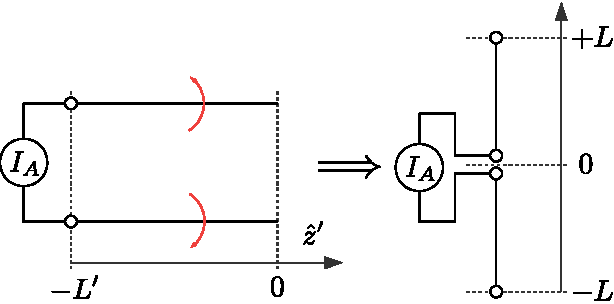
\includegraphics[]{img/linea_antenna_filiforme.pdf}
	\caption{Schema di un antenna filiforme e della linea di trasmissione associata.}
	\label{fig:linea_antenna_filiforme}
\end{figure}

Si può osservare come la linea presenta un circuito aperto ad una delle estremità: esso può essere modellizzato ponendo un carico $Z_L$ con impedenza puramente reale e infinita.

Il campo elettrico non si propaga quindi nello spazio esterno al circuito: le sue linee di forza escono infatti da un filo e rientrano nell'altro.

Se però apriamo i due fili, come in figura, il campo elettromagnetico non rimarrà confinato, non permettendo la chiusura delle linee di campo: ci sarà perciò irraggiamento, pur mantenendo una distribuzione di corrente simile.

\bigbreak
La propagazione di un'onda di tensione lungo la linea si può descrivere con queste leggi, che risultano, con le componenti progressiva e regressiva, analoghe a quelle delle onde piane.
\begin{esp}\begin{dcases}
	V(z^{\prime})=V_+ \, e^{-\jmath\beta z^{\prime}} + V_- \, e^{\jmath\beta z^{\prime}}\\
	I(z^{\prime})=I_+ \, e^{-\jmath\beta z^{\prime}} - I_- \, e^{\jmath\beta z^{\prime}}
\end{dcases}\end{esp}

Nel caso di circuito aperto ($Z_L \to +\infty$) il coefficiente di riflessione risulta chiaramente $\rho = 1$, perciò le due onde progressiva e regressiva hanno uguale ampiezza.

La corrente lungo la linea risulta quindi

\begin{equation*}
	I(z^{\prime})
	= I_+(e^{-\jmath\beta z^{\prime}} - e^{\jmath\beta z^{\prime}})
	= -2j \, I_+ \sin (\beta z^{\prime})
\end{equation*}

Individuiamo come condizione al contorno la corrente ai capi del generatore: è quindi possibile ricavare l'espressione generale per $I$.

\begin{esp}\label{eq:I_fili}
	I(-L^{\prime})&=	I_A = +2j \, I_+ \sin (\beta L^{\prime}) \\
	\implies & I_+ = \frac{I_A}{+2\jmath\sin (\beta L^{\prime})}\\
	\implies & I(z^{\prime}) - \frac{I_A\, \sin (\beta z^{\prime})}{\sin (\beta L^{\prime})}	= - I_m \sin (\beta z^{\prime})
\end{esp}
dove $I_m = {I_A} / \sin (\beta L^{\prime})$ è la corrente massima.

\bigbreak
Possiamo agevolmente passare dal sistema di riferimento della linea a quello dell'antenna con questa trasformazione.
\begin{equation}
 \forall z \in [-L^{\prime}, L^{\prime}], \quad z^{\prime} = \left | z \right | - L^{\prime}
\end{equation}

L'equazione \eqref{eq:I_fili} si può quindi riscrivere, per $|z| \le L/2$, come
\begin{esp}
	I(z)
	& = -I_m \, \sin (\beta \, (|z| - L^{\prime}))
	= I_m \, \sin \left(
		\beta \left(
			\frac{L}{2} - |z|
		\right)
	\right) \\
	& = I_A \,
	\frac {\sin \left(
		\beta \left(
			\frac{L}{2} - |z|
		\right)
	\right)} {\sin \left( \beta \, \frac{L}{2}\right)}
\end{esp}

Il modello della linea approssima molto bene la distribuzione di corrente dell'antenna, ma così non si può dire per l'impedenza.

Il suo valore nella linea è puramente immaginario (infatti essa non irradia) mentre sappiamo che un'antenna irradia solamente se $R_A \neq 0$.
\begin{equation}
	Z(z^{\prime}) = \frac{V(z^{\prime})}{I(z^{\prime})} \propto \jmath \ctg( \beta z^{\prime})
\end{equation}

$Z_A$ non potrà quindi essere ricavata con questa utile approssimazione, ma attraverso tecniche più complesse e precise.

\section{Dipolo corto (o antenna corta)}

Il dipolo corto è la realizzazione fisica più vicina al dipolo elementare.
La sua lunghezza non è ovviamente infinitesima, ma solamente molto inferiore alla lunghezza d'onda della comunicazione.

Data $L$ la lunghezza del dipolo, possiamo quindi scrivere questa proprietà come
\begin{equation}
	\beta L \ll 1
	\Longleftrightarrow \frac{2 \pi}{\lambda} L \ll 1
	\implies L \ll \frac{\lambda}{2 \pi}
\end{equation}

La distribuzione di corrente dell'antenna corta si può calcolare come
\begin{equation} \label{eq:corrente_dipolo_corto}
	I(z)
	= I_A \,
	\frac {\sin \left(
		\beta \left(
			\frac{L}{2} - |z|
		\right)
	\right)} {\sin \left( \beta \, \frac{L}{2}\right)}
	\stackrel{(*)}{\simeq} I_A \,
	\frac {\beta \left(
			\frac{L}{2} - |z|
		\right)} {\beta \, \frac{L}{2}}
	= I_A \, \left(
			1 - \frac{2 |z|}{L}
	\right)
\end{equation}
dove in (*) è applicata l'approssimazione di Taylor, siccome $\beta L \ge \beta |z|$ è infinitesimo.

Una volta ottenuta $I(z)$ è possibile applicare \autoref{eq:A_generico} per ottenere tutte le informazioni riguardo l'irraggiamento dell'antenna in campo lontano, a partire dal potenziale vettore magnetico.
\begin{esp}
	\vec{A}(\rp)
	&= \frac{\mu}{4\pi} \,
	\frac{\ejbr}{r} \,M(\theta, \phi) \\
	&= \frac{\mu}{4\pi} \,
	\frac{\ejbr}{r} \hhat{z} \int_{-\frac{L}{2}}^{\frac{L}{2}} I(z^\prime) e^{\jmath\beta z^\prime \cos (\phi (z^\prime))} \de z^{\prime} \\
	&\stackrel{(1)}{\simeq} \frac{\mu}{4\pi} \frac{e^{-\jmath\beta r}}{r} \hhat{z} \int_{-\frac{L}{2}}^{\frac{L}{2}} I(z^{\prime})\de z^{\prime} \\
	&\stackrel{(2)}{\simeq} \frac{\mu}{4\pi} \frac{e^{-\jmath\beta r}}{r} \hhat{z} \int_{-\frac{L}{2}}^{\frac{L}{2}} I_A \left(1-\frac{2 |z|}{L} \right) \de z^{\prime} \\
\end{esp}
dove in (1) il termine di fase si trascura, perché nel dipolo corto $\beta z^\prime \simeq 0$, mentre in (2) si applica l'approssimazione trovata in \autoref{eq:corrente_dipolo_corto}.

L'ultimo termine si può calcolare come
\begin{esp}
	M(\theta, \phi)
	& = \hhat{z} \int_{-\frac{L}{2}}^{\frac{L}{2}} I_A \left(1-\frac{2 |z|}{L} \right) \de z^{\prime} \\
	& = I_A \left[
		\int_{-\frac{L}{2}}^{\frac{L}{2}}\de z^{\prime} -
		\frac{2}{L} \int_{0}^{\frac{L}{2}} z^\prime \de z^{\prime} +
		\frac{2}{L} \int_{-\frac{L}{2}}^{\,0} z^{\prime} \de z^{\prime}
	\right] \hhat{z}
	= \frac{I_A\, L}{2} \hhat{z}
\end{esp}

Quindi il potenziale magnetico si semplifica a
\begin{esp}
	\A(\r^{\prime})
	&= \frac{\mu}{4\pi} \frac{e^{-j\beta r}}{r} \hat{z}\int_{-\frac{L}{2}}^{\frac{L}{2}} I(z')dz^\prime \\
	&= \frac{\mu}{4\pi} \frac{e^{-j\beta r}}{r} \frac{I_A \, L}{2} \hat{z}
\end{esp}

Questa espressione si differenzia da quella del dipolo elementare, dove manca il fattore 2 al denominatore.
\begin{equation*}
	\A(\r^{\prime})
	= \frac{\mu}{4\pi}
	\frac{e^{-j\beta r}}{r}
	I_A \, \Delta z \hhat{z}
\end{equation*}

\bigbreak
Come fatto per il dipolo elementare, sfruttiamo ora la conoscenza del potenziale vettore magnetico per ricavare campo elettrico e magnetico in campo lontano.
Il procedimento risulta identico, eccetto il fattore 2, al caso elementare, perciò è qui omesso.

\begin{equation}\begin{dcases}
	E_\theta
	\simeq \jmath \eta\,\frac{I}{2\lambda}\, \frac{L}{2} \, \frac{\ejbr}{r} \, \sin(\theta) \\
	H_\theta
	\simeq \jmath \,\frac{I}{2\lambda}\, \frac{L}{2} \, \frac{\ejbr}{r} \, \sin(\theta) \\
\end{dcases}\end{equation}

Di seguito vengono riportati alcuni parametri fondamerntali per il dipolo corto, partendo da quanto definito in sezione \ref{sec:paramAnt}.

\subsection{Parametri d'antenna}

Per il dipolo corto si trova che, analogamente al dipolo elementare,
\begin{equation}
\left | F(\theta, \phi) \right |^2 = \left | \frac{E(r, \theta, \phi)}{E(r, \theta_{MAX}, \phi_{MAX})} \right |^2 = \sin^2\theta
\end{equation}

Possiamo inoltre ricavare le espressioni della potenza irradiata e della resistenza di radiazione, riprendendo i passaggi di \autoref{eq:pot-resRadDE}.

\begin{equation*}
P = \frac{\pi}{3} \eta \left | I_A \right |^2 \left(\frac{L}{2 \lambda}\right)^2 = \frac{\pi}{12} \eta \left | I_A \right |^2 \left(\frac{L}{\lambda}\right)^2
\end{equation*}
\begin{equation*}
R_r = \frac{2}{3} \frac{\pi}{4} \eta \left(\frac{L}{2 \lambda}\right)^2 = \frac{\pi}{6} \eta \left(\frac{L}{2 \lambda}\right)^2 = \frac{\pi}{6} 120 \pi	 \left(\frac{L}{2 \lambda}\right)^2 = 20 (\pi)^2 \left(\frac{L}{2 \lambda}\right)^2
\end{equation*}

Trattandosi di un oggetto filiforme, è possibile definire la \emph{resistenza per unità di lunghezza}.
\begin{equation*}
			r_f = \frac{R_s}{2 \pi a} = \frac{1}{2 \pi a} \sqrt{\frac{\pi f M }{\sigma}}
		\end{equation*}

\section{Dipolo a mezz'onda}

Il dipolo a mezz'onda è un antenna filiforme nella quale ognuno dei due rami è lungo $L = \frac{\lambda}{4}$.

Il suo campo elettrico del dipolo a mezz'onda può essere ricavato con lo stesso procedimento impiegato per il dipolo corto, dove però viene fatta cadere l'approssimazione $\beta \, L \simeq 0$.

Il campo elettrico diventa quindi
\begin{equation*}
	\E
	\simeq \jmath \frac{\eta}{2 \pi} \frac{\ejbr}{r} \frac{I_m \cos \left(\frac{\beta L}{2} \cos \theta \right) - \cos \left(\frac{\beta L}{2} \right)}{\sin \theta} \hth
\end{equation*}

In particolare, siccome $\frac{\beta L}{2} = \frac{\pi}{2}$, si ottiene

\begin{equation}\begin{dcases}
	\E \simeq \jmath \frac{\eta}{2 \pi} \frac{\ejbr}{r} \frac{I_m \cos \left(\frac{\pi}{2} \cos \theta \right)}{\sin \theta} \hth \\
	\H \simeq \frac{E_{\theta}}{\eta} \hphi
\end{dcases}\end{equation}

\subsection{Parametri d'antenna}
Ricaviamo ora i parametri d'antenna trovati sia per il dipolo elementare che per il dipolo corto, nel caso del dipolo a mezz'onda.

\begin{itemize}
	\item Pattern di radiazione in campo
	\begin{equation}
		F(\theta, \Phi) = \frac{\cos \left(\frac{\pi}{2} \cos \theta \right)}{\sin \theta}
	\end{equation}

	\item Pattern di radiazione in potenza
	\begin{equation}
		\left | F(\theta, \phi) \right |^2 = \left | \frac{E(r, \theta, \phi)}{E(r, \theta_{MAX}, \phi_{MAX})} \right |^2 = \frac{\cos^2 \left(\frac{\pi}{2} \cos \theta \right)}{\sin^2 \theta}
		~~ \implies ~~
		\theta_{MAX} = \frac{\pi}{2}
	\end{equation}

	\item Vettore di Poynting
	\begin{equation}
		\P
		= \int_{S(r)} \frac{\E \times \H^*}{2} \de S
		= \int_{S(r)} \frac{\left | E_{\theta} \right |^2}{2 \eta} \de S \hhat{r}
		= \ldots = \frac{C_{in} (2 \pi)}{8 \pi} \eta \left | I_m \right |^2 \hhat{r}
	\end{equation}
	con $C_{in}$ la funzione \emph{coseno integrale}.
	Il valore approssimato del coseno integrale in $2\pi$ è $2,44$.

	\item Resistenza di radiazione

	Dalla sua definizione, $R_r$ si ricava come
	\begin{esp*}
		\Re [\P \cdot \hat{r}]
		& = \frac{C_{in} (2 \pi)}{8 \pi} \eta \left | I_A \right |^2
		= \frac{R_r \left | I_A \right |^2}{2} \\
		R_r
		& = \frac{C_{in} (2 \pi)}{4 \pi} \eta \simeq 73 \Omega
	\end{esp*}

	\item Direttività
	\begin{esp}
		D
		& = \frac{4 \pi r^2 \, I(r, \theta_{MAX}, \phi_{MAX})}{P}
		= \frac{4 \pi r^2 \frac{\left | E_{\theta} \right |^{2}_{MAX}}{2 \eta}}{P}
		= \ldots = \\
		&= \frac{4}{C_{in} (2 \pi)} = \frac{4}{2.44} \cong 1.63
	\end{esp}

	\item Resistenza superficiale del filo
	\begin{equation}
		R_s = \sqrt{\frac{\pi f \mu_0}{\sigma}}
	\end{equation}

	\item Resistenza per unità di lunghezza, dato $a$ il raggio del conduttore
	\begin{equation}
		r_f = \frac{R_s}{2\pi a}
	\end{equation}

	\item Resistenza ohmica
	\begin{equation}
		R_o
		= \frac{2 P_0}{\left |I_A \right |^{2}}
		= \frac{2}{\left |I_A \right |^{2}} \int_{-\frac{L}{2}}^{\frac{L}{2}} r_f \frac{\left |I(z) \right |^{2}}{2} \de z^\prime
	\end{equation}
\end{itemize}

\section{Antenne a lunghezza maggiore di $\frac{\lambda}{2}$}
Per le antenne filiformi con lunghezza superiore a mezza lunghezza d'onda si hanno le caratteristiche elencate nella seguente tabella.

\begin{table}[hb!]
	\centering
	\begin{tabular}{cC{8cm}}
		\toprule
		Lunghezza d'antenna & Note\\
		\midrule
		 \vspace{2mm}
		$\frac{3}{4}\lambda$ & non ha un'impedenza d'ingresso  ``standard'', ovvero compatibile con le linee più comuni \\ \vspace{2mm}
		$\lambda$ & $Z_A \to +\infty$, quindi è difficile da adattare \\
		$>\lambda$ & si introducono lobi secondari: l'antenna perde in direttività \\
		\bottomrule
	\end{tabular}
\end{table}

\section{Yagi-Uda}
Analizzeremo ora il caso di due antenne poste ad una certa distanza $d = \lambda / 4$, l'una attiva e l'altra passiva, come in \autoref{fig:yagi_uda_due_pezzi}.

I due elementi avranno lunghezza $\lambda/2$, per cui la potenza ai loro morsetti risulterà $P_{\lambda/2}\propto \left | I_a \right |^2$ per il trasmettitore e $P_{\lambda/2}\propto (R_r)^{1/2}$ per il ricevitore.

Il primo elemento produce un campo $\E_{driver}$ che incide sul secondo: esso per reazione produce un campo dello stesso modulo ma con segno opposto, chiamato $\E_{parassita} = -\E_{driver}$.

\begin{figure}[htp]
	\centering
	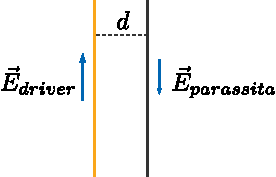
\includegraphics[]{img/yagi_uda_due_pezzi.pdf}
	\caption{L'antenna attiva, in arancione, irradia un campo ``driver'' e aziona l'elemento passivo, in grigio.}
	\label{fig:yagi_uda_due_pezzi}
\end{figure}

Data la distanza $d$, possiamo valutare il modulo campo indotto nel secondo elemento come
\begin{equation}
	E_{parassita}
	= -E_{driver} \,e^{-\jmath \beta d}
	= -E_{driver} \,e^{-\jmath \frac{2 \pi}{\lambda} \frac{\lambda}{4}}
	= -E_{driver} \, e^{-\jmath \frac{\pi}{2}}
\end{equation}

Osserviamo quindi come interagiscono le due antenne nel campo lontano, quindi per $r \gg \lambda$.

Poniamoci a \emph{sinistra} della coppia di antenne, secondo lo schema di \autoref{fig:yagi_uda_due_pezzi}, sommando il contributo dei due elementi.
\begin{esp}
	E
	& \propto E_{driver}\frac{\ejbr}{r}
	-E_{driver}
	\frac {e^{\jmath\beta(r+\frac {\lambda} {4})}} {r}
	\, e^{-\jmath\frac{\pi}{2}} \\
	& = E_{driver} \frac{\ejbr}{r} (1-e^{j (\beta\frac{\lambda}{4} - \frac{\pi}{2})})
	= E_{driver}\frac{\ejbr}{r} (1-e^{-\jmath\pi})
	= 2E_{driver}\frac{\ejbr}{r}
\end{esp}

Il campo elettrico risulta quindi raddoppiato, e in questo caso si parla di interfernza costruttiva.

Analizzando invece il caso di grande distanza a \emph{destra} dell'elemento passivo, il campo elettrico risulta nullo: siamo infatti in presenza di interferenza distruttiva, che rende l'antenna equivalente ad un piano conduttore.

\begin{equation}
	E
	\propto E_{driver} \frac{\ejbr}{r}
	- E_{driver} \frac{e^{-\jmath\beta(r-\frac{\lambda}{4})}}{r} e^{-\jmath\frac{\pi}{2}}
	= E_{driver}\frac{\ejbr}{r} (1-e^{-\jmath\frac{\pi}{2}} e^{\jmath\frac{\pi}{2}})
	= 0
\end{equation}

Le due antenne possono essere viste come un doppio bipolo elettrico, definendo per ciascuna una tensione ai capi $V$ e una corrente in ingresso $I$, legate da una matrice di impedenze.

\begin{equation}
	\left(
		\begin{array}{c}
			V_1 \\
			V_2
		\end{array}
	\right)
	= \left(
		\begin{array}{cc}
			Z_{11} & Z_{12} \\
			Z_{21} & Z_{22}
		\end{array}
	\right)
	\left(
		\begin{array}{cc}
			I_1 \\
			I_2
		\end{array}
	\right)
\end{equation}

Nel componente passivo, vale quindi che
\begin{equation}
	\begin{dcases}
		V_2 = Z_{21}I_1+Z_{22}I_2 = 0 \\
		I_2 = -I_1 \frac{Z_{21}}{Z_{22}}
	\end{dcases}
\end{equation}

% TODO: chiarire: non si capisce nulla
% Nel caso reale:

% nel caso d = 0, la parte reale di $Z_{21}$ è $73\omega$, mentre nel caso $d = 0.15 \lambda$, la parte reale di $Z_{21}$ risulta $63\omega$. Facendi i calcoli con questa ultima distanza, ci si accorge che la corrente $I_{2}$ è circa ddel 10\% (0.89) più bassa di $I_{1}$.

% ...Disegni su campo elettrico in condizioni reali...

\clearpage
\section{Dipolo Magnetico elementare}

Il dipolo magnetico è il duale del dipolo elettrico, ed è composto da una spira infinitesima di lunghezza $\Delta s$ percorsa da una corrente $I$.

Lo studio è analogo a quello del dipolo elettrico, con le dovute sostituzioni riportate nella \autoref{tab:dipolo_elettrico_magnetico}.

\begin{table}[h]
	\centering
	\begin{tabular}{cc}
		\toprule
		Dipolo elettrico & Dipolo magnetico \\
		\midrule
		$E_{\theta}$, $E_{r}$ & $H_{\theta}$, $H_{r}$ \\
		$H_{\phi}$ & $-E_{\phi}$ \\
		$I \Delta z$ & $I^{(m)} \Delta z =  \jmath \omega \mu I \Delta s$ \\
		$\eta$ & $\frac{1}{\eta}$ \\
		\bottomrule
	\end{tabular}
	\caption{Tabella di conversione tra i due dipoli. $I^{(m)}$ nel dipolo magnetico è la corrente magnetica equivalente, definita per simmetria.}
	\label{tab:dipolo_elettrico_magnetico}
\end{table}

I campi elettrico e magnetico possono essere quindi scritti come

\begin{equation}
	\begin{dcases}
		\H
		= \frac{I^{(m)} \Delta z}{4 \pi \eta}
		\left(
			\frac{\jmath \beta}{r} + \frac{1}{r^2}
			+ \frac{1}{\jmath \beta r^3}
		\right)
		\sin (\theta) \, \ejbr \hth
		+ \frac{I^{(m)} \Delta z}{2 \pi \eta}
		\left(
			\frac{1}{r^2} + \frac{1}{\jmath \beta r^3}
		\right)
		\cos (\theta) \, \ejbr \hr \\
		\E
		= - \frac{I^{(m)} \Delta z}{4 \pi}
		\left(
			\frac{\jmath \beta}{r}
			+ \frac{1}{r^2}
			+ \frac{1}{\jmath \beta r^3}
		\right)
		\sin (\theta) \, \ejbr \hphi
	\end{dcases}
\end{equation}
con $I^{(m)} \Delta z = \jmath \omega \mu I \Delta s$.

Nel caso di campo lontano ($r \gg \lambda$) i due campi, elettrico e magnetico, si semplificano come segue
\begin{equation}
	\begin{cases}
		\begin{split}
			\H
			\simeq H_{\theta} \hth
			& = \frac{\jmath \omega \mu I \Delta s}{4 \pi \eta} \frac{\jmath \beta}{r} \sin (\theta) \, \ejbr \hth
			= -\frac{\omega \mu I \Delta s}{4 \pi \sqrt{\frac{\mu}{\epsilon}}}
			\, \omega \sqrt{\mu \epsilon} \sin (\theta)
			\, \frac{\ejbr}{r} \hth \\
			& = -\frac{\pi I \Delta s}{\lambda^2} \sin (\theta)\, \frac{\ejbr}{r} \hth
		\end{split} \\
		E_{\phi} = - \eta H_{\theta}
	\end{cases}
\end{equation}

Il pattern di radiazione invece risulta uguale a quello del dipolo elementare, così come la direttività, sempre pari a $1.5$.

\begin{equation}
	F(\theta, \phi)
	= \frac{E(r, \theta, \phi)}{E(r, \theta_{MAX}, \phi_{MAX})} = \sin(\theta)
\end{equation}

La potenza in uscita si rivela essere
\begin{equation*}
	P
	= \Re \left[
		\int_{S(r)} \frac{\E \times \H^*}{2}
	\right]
	= \ldots
	= 10 |I|^2 \, \left(
		\frac{4\pi^2 \Delta s}{\lambda^2}
	\right)^2
	= \frac{1}{2} |I|^2 R_r
\end{equation*}
dove si è ricavata anche la resistenza di radiazione $R_r$.

Come per il dipolo elementare elettrico, anche qui l'antenna risulta di difficile utilizzo, sia in termini di potenza irradiata che di adattabilità alla linea.

\section{Antenna a Banda Larga}
% TODO: mettere giù per bene
- elica, come schiera fasata di spire lunghe $2\pi b$

- antenna biconica

- antenna log-periodica, composta da segmenti con frequenze in progressione geometrica

%%% Local Variables:
%%% mode: latex
%%% TeX-master: "antenne"
%%% End:
